\documentclass[UTF8]{ctexart}
\usepackage{amsmath}
\usepackage{geometry}
\usepackage{graphicx}
\usepackage{gensymb}
\usepackage{wrapfig}
\usepackage{titlesec}
\usepackage{float}
\usepackage{diagbox}
\geometry{a4paper,scale=0.8}
\titlespacing*{\section}
{0pt}{0pt}{0pt}
\titlespacing*{\subsection}
{0pt}{0pt}{0pt}
\titlespacing*{\paragraph}
{0pt}{0pt}{0pt}
\titlespacing*{\subparagraph}
{0pt}{0pt}{0pt}
\CTEXsetup[format+={\raggedright}]{section} 
\CTEXsetup[format+={\raggedright}]{subsection} 
\title{弹簧振子实验}
\author{Deschain}
\begin{document}
\maketitle
\section*{一、实验目的}
1.观测简谐振动的特点\\
2.掌握质量、时间、长度等基本量的测量方法\\
3.联系并掌握最小二乘法直线拟合\\
\section*{二、实验原理}
\paragraph{}
质量为$m$的物体悬挂在劲度系数为$k$、上端固定的轻质弹簧下端。在弹簧弹性形变范围内给定一个偏离,使物体沿竖直方向上下振动,即形成弹簧振子。定义振子运动位移沿竖直方向为x轴,向下为正,且振子受合力为零的平衡处$x=0$,同时振子所受合力$F$、运动速度$v$均沿竖直方向,向下为正。\\
可以证明振子会做简谐振动:\\
$x=Acos(\omega t+\varphi_0)$\\
振动固有角频率$\omega$由系统本身的性质决定:\\
$\omega=\sqrt{\frac{k}{m}}$\\
弹簧振动周期$T$的公式为:\\
$T=2\pi\sqrt{\frac{m}{k}}$\\
考虑到弹簧质量$m_0$的影响后,弹簧振子振动周期公式修正为:\\
$T=2\pi\sqrt{\frac{m+cm_0}{k}}$\\
其中c为与弹簧形状、质量分布等因素有关的系数。\\
上式可变形为:\\
$T^2=\frac{4\pi^2}{k}m+\frac{4\pi^2cm_0}{k}$\\
实验中使用一根弹簧,通过测量振子取不同砝码质量$m$时的振动周期$T$,拟合$T-m$直线,即可由斜率得出弹簧劲度系数k,由截距和斜率得出弹簧等效质量系数$c$。\\
上式还可变形为:\\
$lnT=ln(2\pi\sqrt{m+cm_0})-\frac{lnk}{2}$\\
通过保持振子质量$m$不变,选取不同$k$的弹簧,测量振动周期,拟合$lnT-lnk$直线,验证其斜率为-0.5(假定各弹簧质量差别不大,$m_0$取不同弹簧质量的平均值)。\\
\section*{三、实验仪器及使用说明}
支架,弹簧,钩码,砝码,秒表,电子天平,数显高度尺。\\
1.秒表:最小分度值为0.01s。\\
2.电子天平:使用前先调平、去皮归零。使用时勿撞击秤盘,以免损坏仪器。\\
3.数显高度尺。\\
\section*{四、实验任务、步骤及注意事项}
注:本实验中的周期测量指测50个周期,测三次,取平均。\\
1.测量6个弹簧的质量及钩码、各个砝码的质量\\
2.拉伸法测量6组弹簧的劲度系数\\
3.测量某一弹簧的振动周期,计算$k$和$c$。\\
(1)掌握停表测量振动周期技巧。\\
(2)探究振动幅度与周期的关系。\\
保持振子质量不变,改变振子的最大初始振幅$A$,(分别取$20mm$,$25mm$,$30mm$),测量弹簧振动周期,观测周期是否改变。同时观测50个周期中振幅的变化。根据观测结果确定合适的初始最大振幅。\\
(3)测量不同振子质量下的振动周期T,计算$k$和$c$。\\
保持弹簧振子的最大初始振幅不变,依次添加7个砝码,记录振子总质量,并测量其振动周期。利用测量得到的数据拟合$T^2-m$直线,并利用拟合的斜率和截距计算$k$,$c$,并与任务2中得出的该弹簧的劲度系数k作比较。\\
4.固定振子质量,改变弹簧劲度系数测周期,验证$T-k$的关系\\
通过实验验证$lnT-lnk$直线关系的斜率与-0.5是否相符。$m_0$取各个弹簧质量的平均值,砝码振子的质量$m$应尽量大。保持弹簧振子的质量不变,测量6个弹簧的简谐振动周期。\\
\section*{五、实验数据处理}
\subsection*{1.质量测量}
\begin{tabular}{|l|l|l|l|l|l|l|}
\hline
编号 &1(最细)&2(红) &3(黄)&4(橙)&5(蓝)&6(最粗)\\
\hline 
弹簧质量/g &30.2360&32.8836&34.9088&39.0922&40.8601&44.1443\\
\hline
\end{tabular}
\newline
\begin{tabular}{|l|l|l|l|l|l|l|l|}
\hline
编号 &1&2&3&4&5&6&7\\
\hline 
砝码质量/g &9.9726&9.8741&9.9636&9.9413&9.9717&9.8651&9.7645\\
\hline
\end{tabular}
\\
钩码质量为41.9243g
\subsection*{2.劲度系数的测量}
\begin{tabular}{|l|l|l|l|l|l|l|l|}
\hline
\diagbox{伸长量/mm}{弹簧编号}&1&2&3&4&5&6&受力/N\\
\hline
$y_1$&7.70&8.18&11.05&13.54&16.20&20.71&0.09773\\
\hline
$y_2$&14.91&17.44&23.13&29.98&35.50&42.69&0.1945\\
\hline
$y_3$&21.87&27.16&37.10&43.81&52.50&64.27&0.2921\\
\hline
$y_4$&29.16&35.59&47.20&59.38&69.15&87.15&0.3896\\
\hline
$y_5$&35.51&43.78&60.30&73.29&88.03&111.27&0.4873\\
\hline
$y_6$&42.36&53.26&73.72&89.35&106.02&131.24&0.5840\\
\hline
\end{tabular}
\newline
$y_1$是在挂有钩码的基础上,添加1号砝码测得的伸长量;$y_2$是挂有钩码、1号砝码、2号砝码测得的伸长量;以此类推。\\
拟合直线(自下至上依次为弹簧1至6):
\begin{figure}[h]
\centering
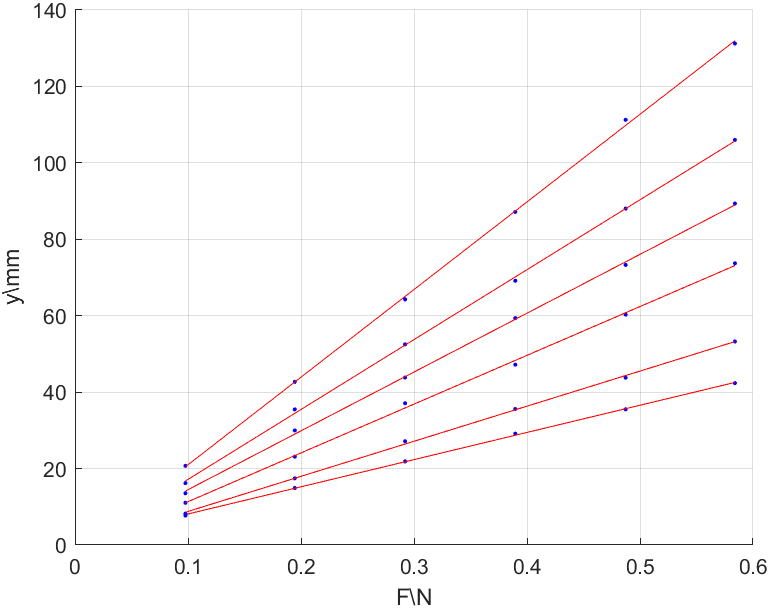
\includegraphics[width=6cm,height=4cm]{exp1.png}
\end{figure}
\begin{equation*}
\begin{aligned}
&y_1=71.14F+1.002, k_1=71.14mm/N, R_2=0.9996\\
&y_2=91.82F-0.396, k_2=91.82mm/N, R_2=0.9992\\
&y_3=127.7F-1.431, k_3=127.7mm/N, R_2=0.9987\\
&y_4=153.9F-0.9175, k_4=153.9mm/N, R_2=0.9994\\
&y_5=182.9F-1.126, k_5=182.9mm/N, R_2=0.9994\\
&y_6=229.3F-1.941, k_6=229.3mm/N, R_2=0.9996\\
\end{aligned}
\end{equation*}
\subsection*{3.测量某一弹簧的振动周期,计算弹簧劲度系数k,弹簧等效质量系数c}
(1)探究振动幅度与周期的关系\\
注:这里记录的是单个周期的时间,50个周期的原始数据见原始数据表格。\\
选择6号弹簧,振子为钩码和1号砝码。\\
\begin{tabular}{|l|l|l|l|l|}
\hline
\quad&第一次测量&第二次测量&第三次测量&平均值\\
\hline
振幅20mm&0.7724&0.7750&0.7730&0.7735\\
\hline
振幅25mm&0.7726&0.7744&0.7750&0.7740\\
\hline
振幅30mm&0.7750&0.7742&0.7744&0.7745\\
\hline
\end{tabular}
\newline
在误差允许的范围内,可以认为振幅与周期无关。\\
(2)选用6号弹簧,振幅30mm\\
\begin{tabular}{|l|l|l|l|l|l|}
\hline
\diagbox{振子质量/g}{周期}&第一次测量&第二次测量&第三次测量&平均值T&$T^2$\\
\hline
54.1169&0.7742&0.7750&0.7744&0.7745&0.5999\\
\hline
64.1040&0.8268&0.8368&0.8286&0.8274&0.6846\\
\hline
74.0676&0.8800&0.8776&0.8780&0.8779&0.7707\\
\hline
84.0089&0.9268&0.9350&0.9274&0.9264&0.8582\\
\hline
93.9806&0.9730&0.9744&0.9724&0.9733&0.9473\\
\hline
103.8457&1.0186&1.0198&1.0176&1.0187&1.0378\\
\hline
113.6102&1.0582&1.0593&1.0600&1.0592&1.1219\\
\hline
\end{tabular}
\newline
拟合曲线:(m的单位是kg,T的单位是s)
\begin{figure}[H]
\centering
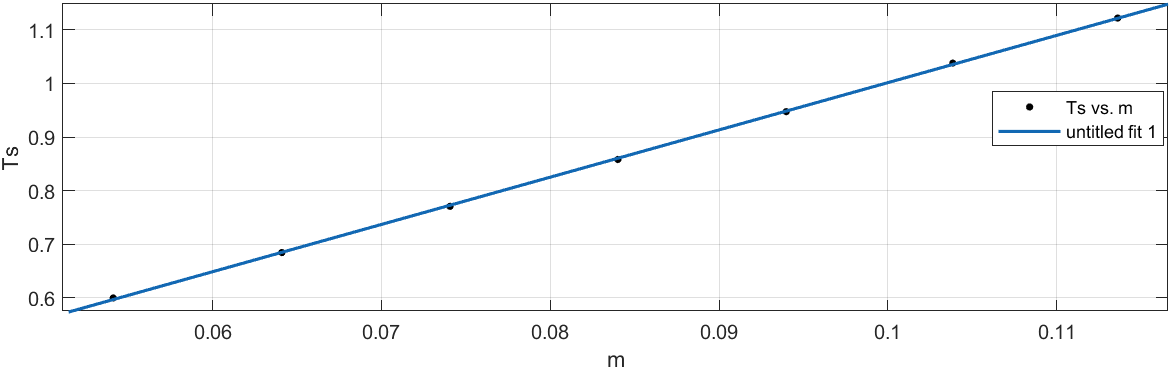
\includegraphics[width=6cm,height=4cm]{exp2.png}
\end{figure}
\begin{equation*}
T^2=8.813m+0.1201,R^2=0.9999
\end{equation*}
\begin{equation*}
\begin{aligned}
&T^2=\frac{4\pi^2}{k}m+\frac{4\pi_2cm_0}{k} = k_1m+b\\
&k=\frac{4\pi^2}{k_1}=4.480N/m\\
&c=\frac{b}{k_1m_0}=0.3087
\end{aligned}
\end{equation*}
\subsection*{4.固定振子质量,改变弹簧劲度系数测周期,验证T-k的关系}
注:振子为钩码和7个砝码,振幅30mm\\
\begin{tabular}{|l|l|l|l|l|}
\hline
\diagbox{弹簧编号}{振动周期}&第一次测量&第二次测量&第三次测量&平均值\\
\hline
1&0.5862&0.5888&0.5870&0.5873\\
\hline
2&0.6744&0.6736&0.6738&0.6739\\
\hline
3&0.7780&0.7782&0.7774&0.7779\\
\hline
4&0.8690&0.8700&0.8694&0.8695\\
\hline
5&0.9450&0.9450&0.9448&0.9449\\
\hline
6&1.0568&1.0580&1.0578&1.0575\\
\hline
\end{tabular}
\newline
\begin{tabular}{|l|l|l|l|l|l|l|}
\hline
ln(k)&2.6431&2.3879&2.0581&1.8715&1.6988&1.4727\\
\hline
ln(T)&-0.5322&-0.3947&-0.2512&-0.1398&-0.0567&0.0559\\
\hline
\end{tabular}
\begin{figure}[H]
\centering
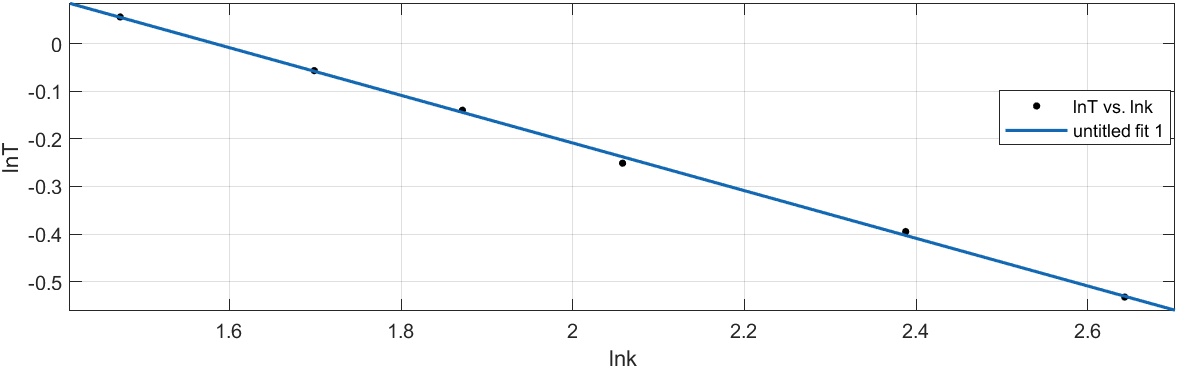
\includegraphics[width=6cm,height=4cm]{exp3.png}
\end{figure}
拟合直线的斜率为-0.5005,截距0.7922,$R^2=0.9989$。在误差允许的范围内,可以认为本实验验证了$lnT=ln(2\pi\sqrt{m+cm_0})-\frac{lnk}{2}$。\\
c的计算:
\begin{equation*}
\begin{aligned}
&m=\sum{m_{fama}}+m_{gouma}=113.6102g=0.1136kg\\
&m_0=\frac{1}{6}\sum{m_i}=37.0208g=0.0370kg\\
&b=ln(2\pi\sqrt{m+cm_0})\\
&c=\frac{(\frac{e^b}{2\pi})^2-m}{m_0}=0.2677
\end{aligned}
\end{equation*}
\section*{六、思考题}
\textbf{1.理论推导均质柱状弹簧等效质量系数c,并比较实验值与理论值。}
\newline
设弹簧质量为m,原长为L,形变均匀,且末端速度为v,则总动能为$E_{k_0}=\int_0^L 0.5\frac{m}{L}(\frac{v}{L}x)^2dx=\frac{1}{6}m_0v^2$,而重物动能为$E_{k_1}=\frac{1}{2}Mv^2$,故$c=\frac{1}{3}$。\\
理论值与实验值差距较大,说明实验时测量的精度不足,误差太大。\\
\textbf{2.实验3中为何选取较粗的弹簧?}
\newline
较粗的弹簧劲度系数较小,周期较大,在振幅相同的情况下,移动速度较慢,便于测量。\\
\textbf{3.计数起停的最佳时机是什么?如何操作可以减少弹簧的左右摆动?}
\newline
(1)人眼判断的是位置,秒表记录的是时间。在相同的位置误差下,速度越快,时间误差越小。所以计数起停的最佳时机是振子运动速度最快时,也就是弹簧振子越过平衡位置时。\\
(2)用双手将弹簧下压一定距离,双手同时松开,这样左右摆动最小。\\
\textbf{4.测量不同振子质量下的周期时,振幅选为多少较为合适?为什么?}
\newline
对于本次实验使用的弹簧,振幅30mm最为合适,因为在30mm下测量结果最为稳定。\\
\textbf{5.拉伸法求得劲度系数k的不确定度如何计算?}
\begin{equation*}
\begin{aligned}
&k=\frac{1}{b}\\
&\Delta_k=\frac{1}{b^2}\Delta_b\\
&\Delta_b=t_p(n-2)S_b=t_p(n-2)\sqrt{\frac{r^{-2}-1}{n-2}}\\
&\Delta_a=t_p(n-2)S_a=t_p(n-2)S_b\sqrt{\frac{\sum{x_i^2}}{n}}\\
&k=\frac{4\pi^2}{b}\\
&\Delta_k=\frac{4\pi^2}{b^2}\Delta_b\\
&c=\frac{1}{M}\frac{a}{b}\\
&\Delta_c=\frac{1}{M}\sqrt{\frac{1}{b^2}\Delta_a{2}+\frac{a^2}{b^4}\Delta_b^2}
\end{aligned}
\end{equation*}
\section*{七、实验小结}
本次实验中,我对“原始数据”有了更为准确的认识。测量周期时,我记录的是单个周期的时间,也就是对原始数据直接除以50再记录。在老师的指导下,我意识到这么做是错误的,原始数据是不应该经过运算处理的。幸好本次实验中测量的是50个周期,可以将原始数据无损还原。认识到这一点,对我今后的实验很有意义,防止未来实验中的数据遭到不可逆的损坏。
\section*{八、原始数据表格}
见附件。

\end{document}